% \documentclass{beamer}
\documentclass[handout]{beamer}
% \documentclass[handout, notes]{beamer}
% \documentclass[handout, notes=only]{beamer}

\usetheme{metropolis}
\setbeamercovered{transparent}
\setbeamertemplate{section in toc}[sections numbered]

\usepackage{amsmath, amssymb, amsthm}
\usepackage{graphicx}
\usepackage{subfigure}
\usepackage[scr]{rsfso}

\def\C{\mathbb{C}}
\def\R{\mathbb{R}}
\def\Q{\mathbb{Q}}
\def\Z{\mathbb{Z}}
\def\N{\mathbb{N}}

\title{
    The Three Classical Problems
    % Three Greek Problems of Antiquity
}
\subtitle{
    An Introduction to Constructible Numbers
}
\author{Satvik Saha}
\institute{
    Department of Mathematics and Statistics, \\
    Indian Institute of Science Education and Research, Kolkata
}
\date{25 February, 2023}

\begin{document}
    \maketitle

    % \section{Classical Conundrums}

    \begin{frame}{The Three Classical Problems}
        \begin{enumerate}
            \item Angle trisection.
            \uncover<2->{\alert{$\pi/9$}}
            \item Doubling the cube.
            \uncover<2->{\alert{$\sqrt[3]{2}$}}
            \item Squaring the circle.
            \uncover<2->{\alert{$\sqrt{\pi}$}}
        \end{enumerate}
    \end{frame}

    \note[itemize]{
        \item Constructing $\pi/9$ would allow the construction of a regular nonagon.

        \item Existing methods of solving these problems.
        \begin{itemize}
            \item Origami
            \item Archimedes' neusis, using a marked ruler
            \item Archimedean spiral
            \item Linkages
            \item A set square
        \end{itemize}

        \item First proved to be impossible by Pierre Wantzel in 1837.
    }

    \begin{frame}
        \begin{figure}
        \begin{center}
            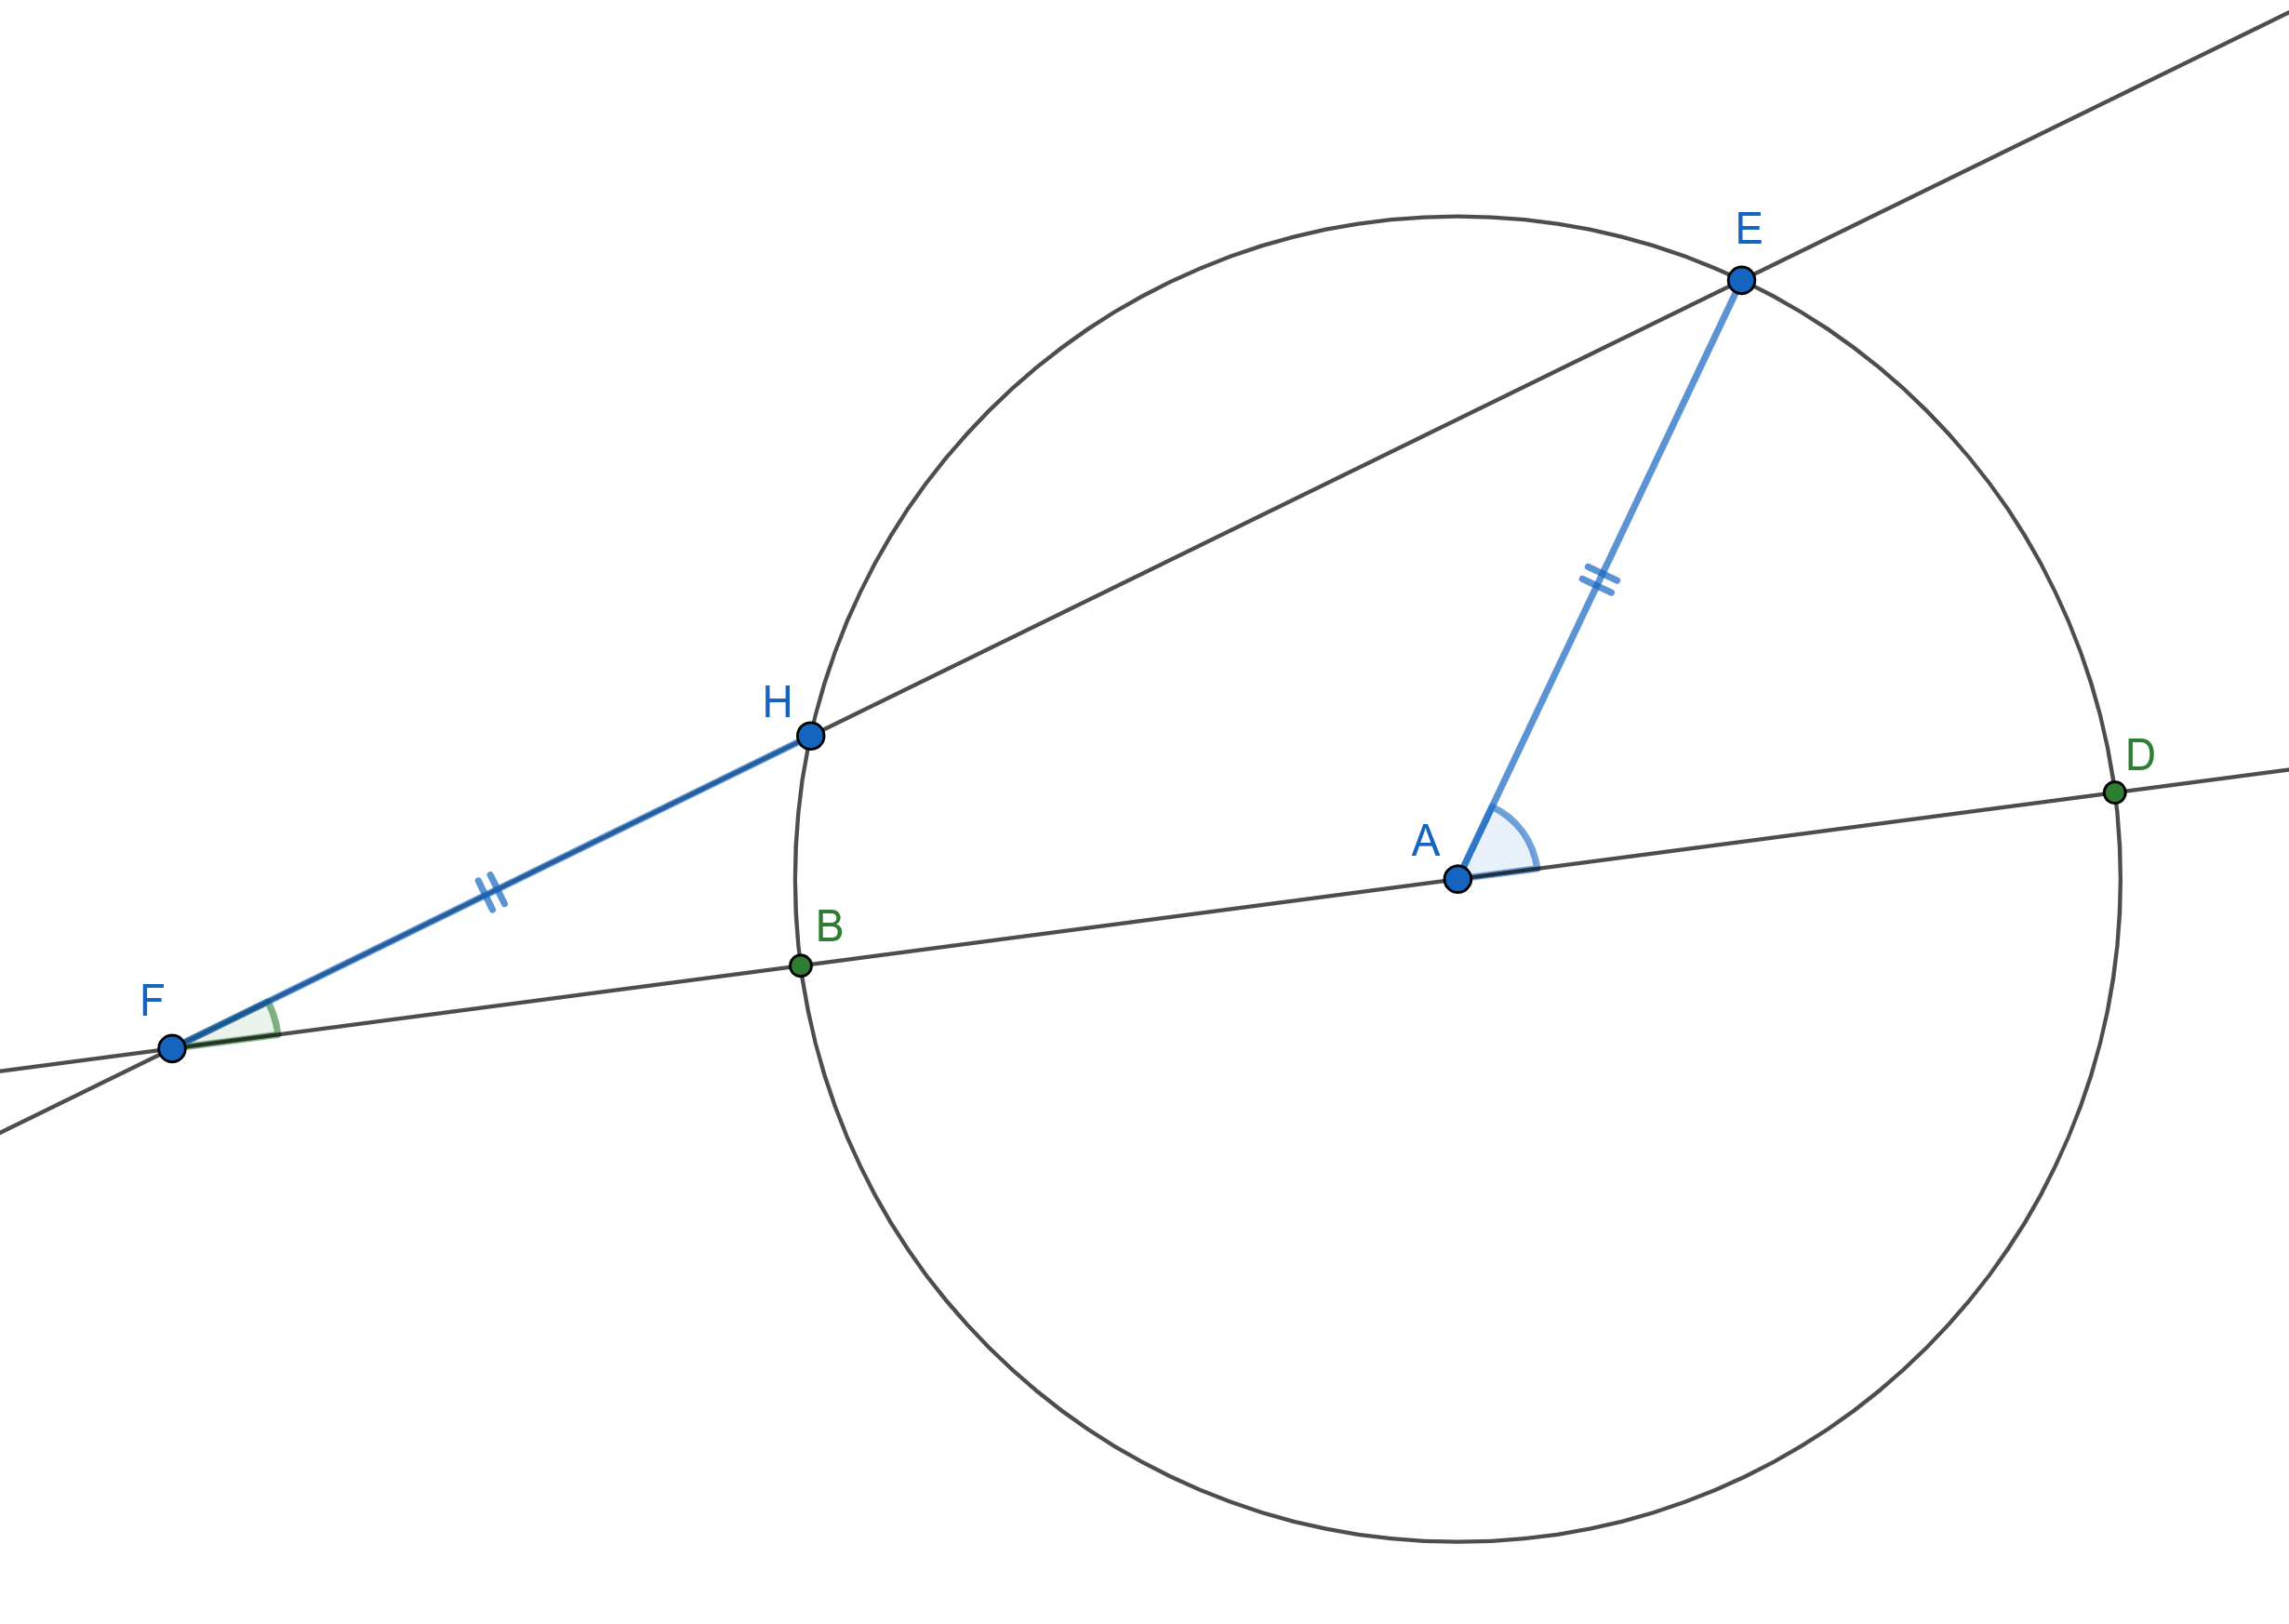
\includegraphics[width=\textwidth]{trisection_archimedes_.png}
        \end{center}
        \caption{Archimedes' method of trisecting an angle.}
        \label{fig:trisecting_angles}
        \end{figure}
    \end{frame}

    \begin{frame}{Outline}
        \tableofcontents
    \end{frame}

    \note[itemize]{
        \item These are non-existence problems; on a scale from the irrationality of
        $\sqrt{2}$ to Fermat's Last Theorem.

        \item Relation to the insolvability of the quintic.

        \item Tools of algebra are used here to resolve this problem in geometry;
        parallel with how the Fundamental Theorem of Algebra can be resolved using
        tools of topology/complex analysis.

        \item Proof on Terry Tao's blog which bypasses the approach using field
        extensions.

        \item Intended as a gentle/motivated introduction to field theory.
    }

    \section{The Rules of the Game}

    \begin{frame}{Straightedge and compass}
        \begin{enumerate}
            \item A line can be drawn through any two constructed points.
            \uncover<2->{\alert{$L(\alpha, \beta)$}}
            \item A circle can be drawn centred at any constructed point, and with
            any previously constructed length as radius.
            \uncover<2->{\alert{$C(\gamma, R)$}}
        \end{enumerate}
        \pause
        The intersection points of constructed lines and circles are added to the
        collection of constructed points.
    \end{frame}

    \begin{frame}
        \begin{figure}
        \begin{center}
            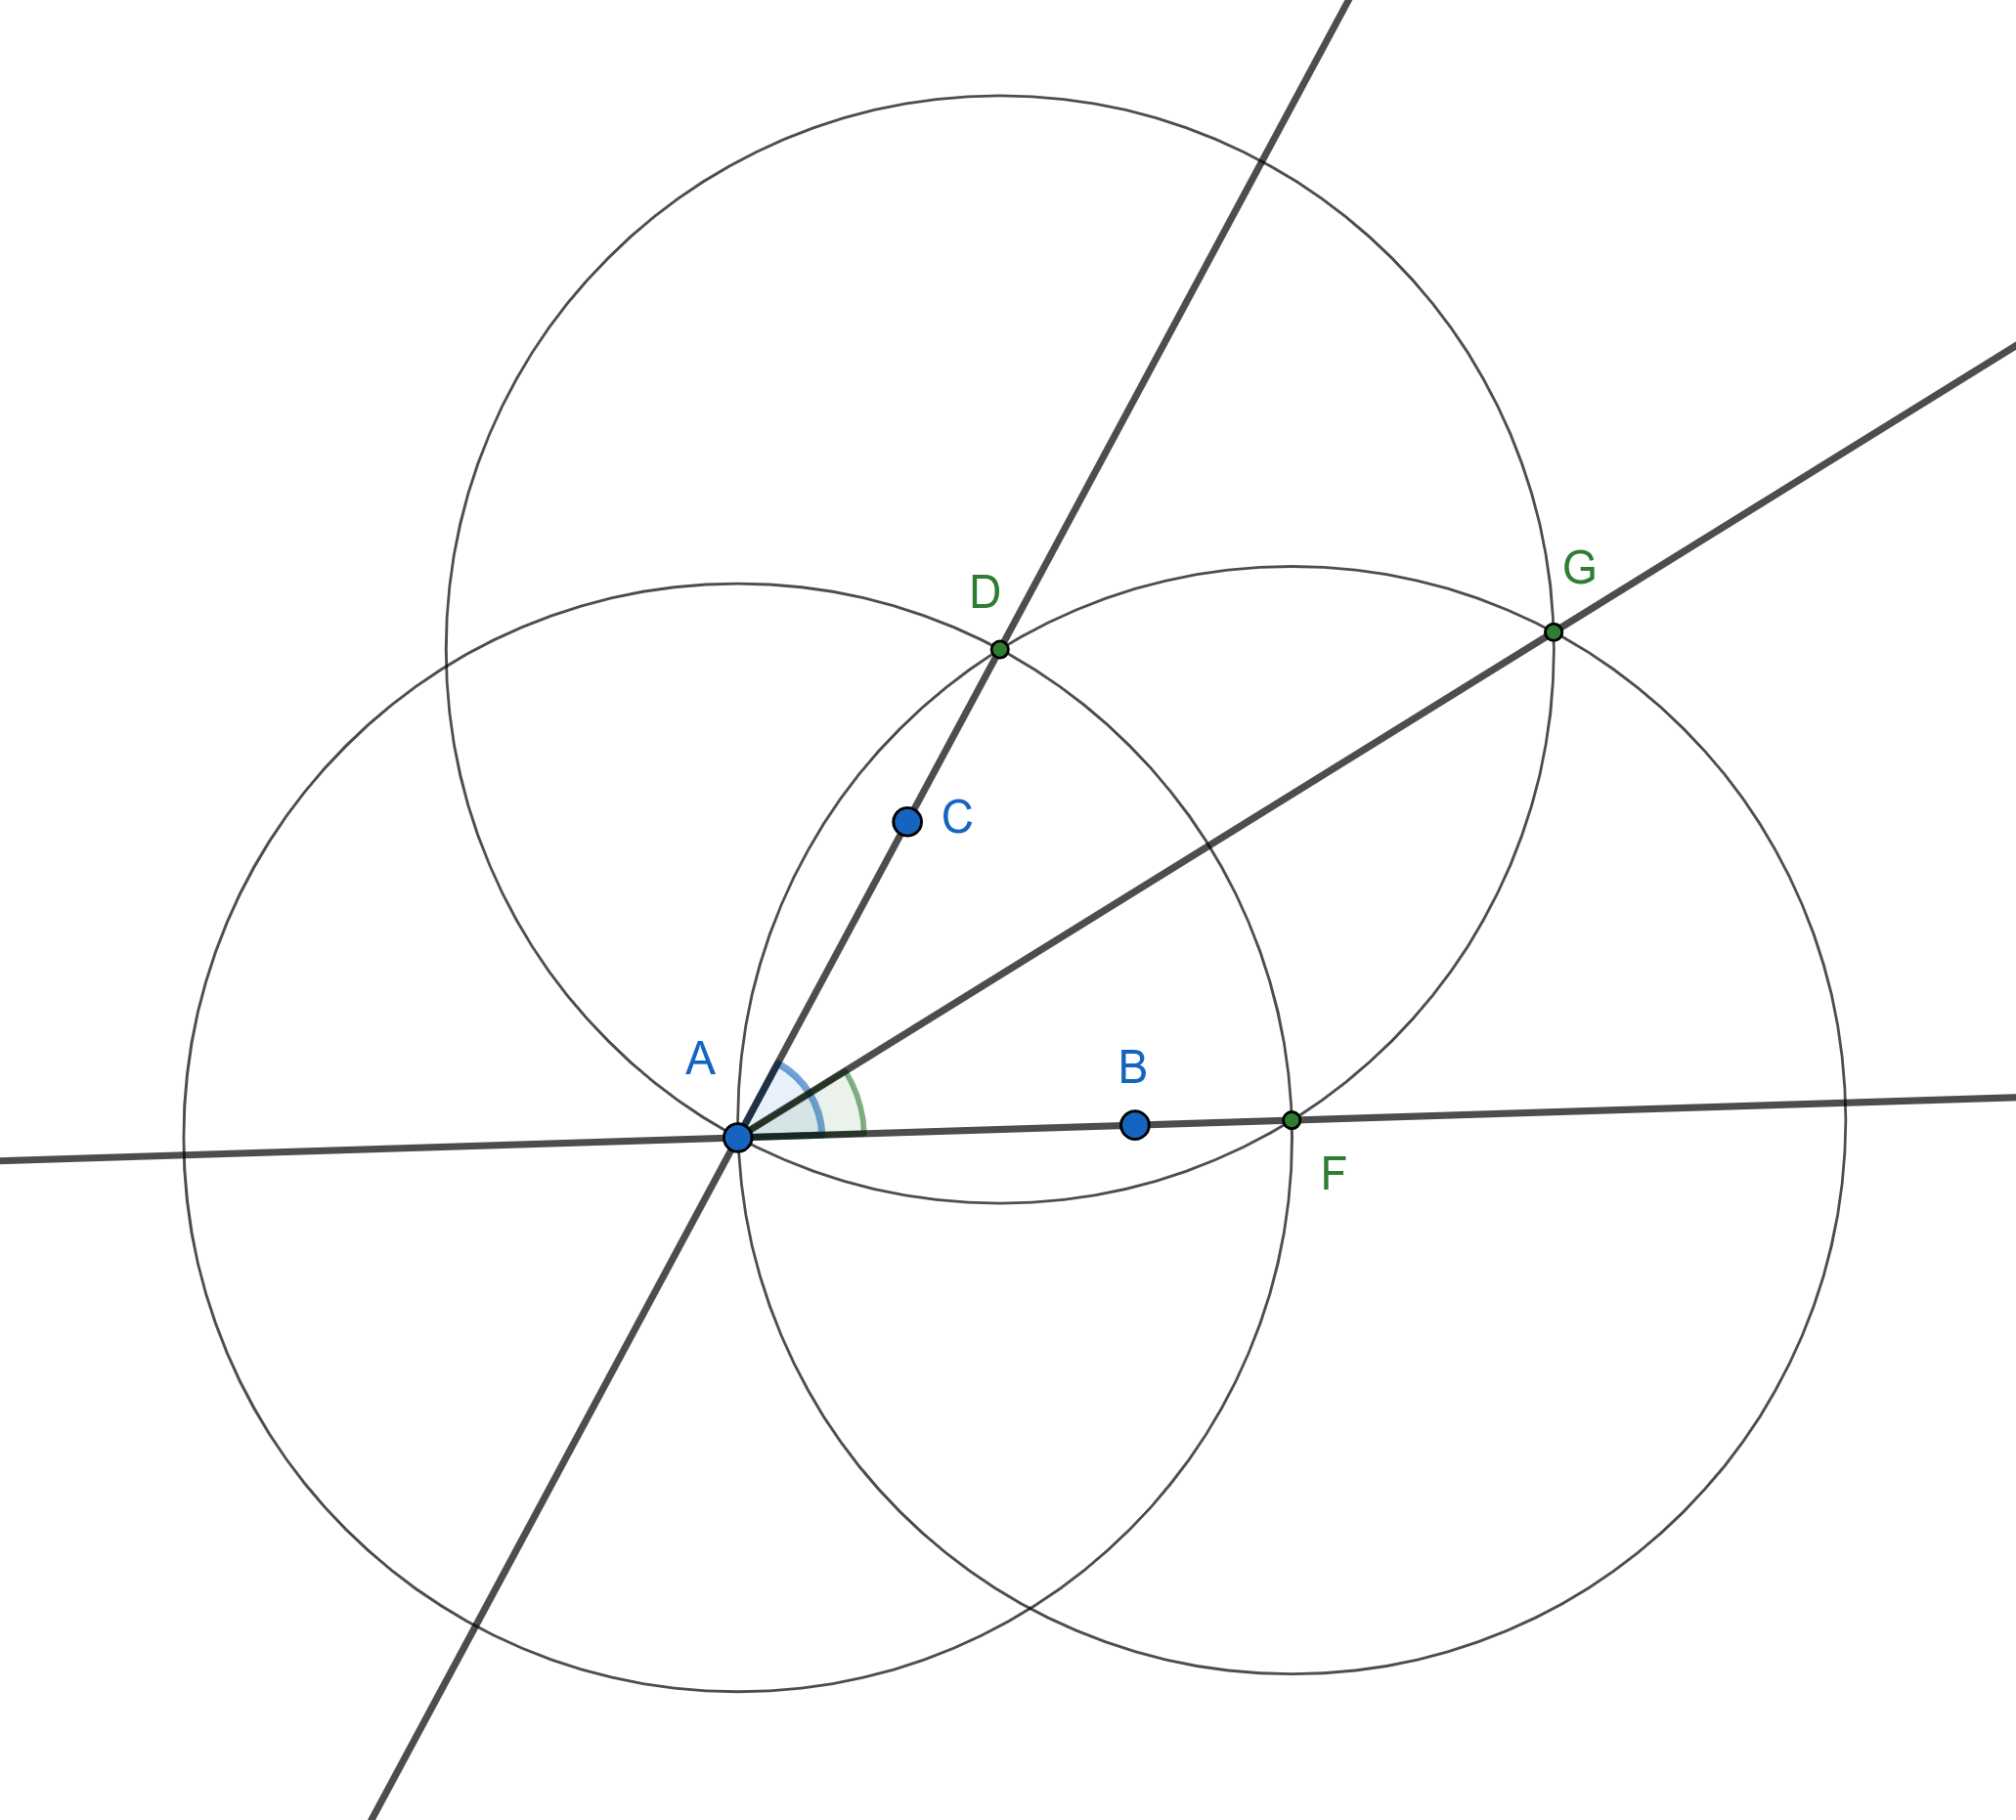
\includegraphics[width=0.75\textwidth]{bisector_.png}
        \end{center}
        \caption{Any angle can be bisected.}
        \label{fig:bisecting_angles}
        \end{figure}
    \end{frame}

    \begin{frame}
        \begin{figure}
        \begin{center}
            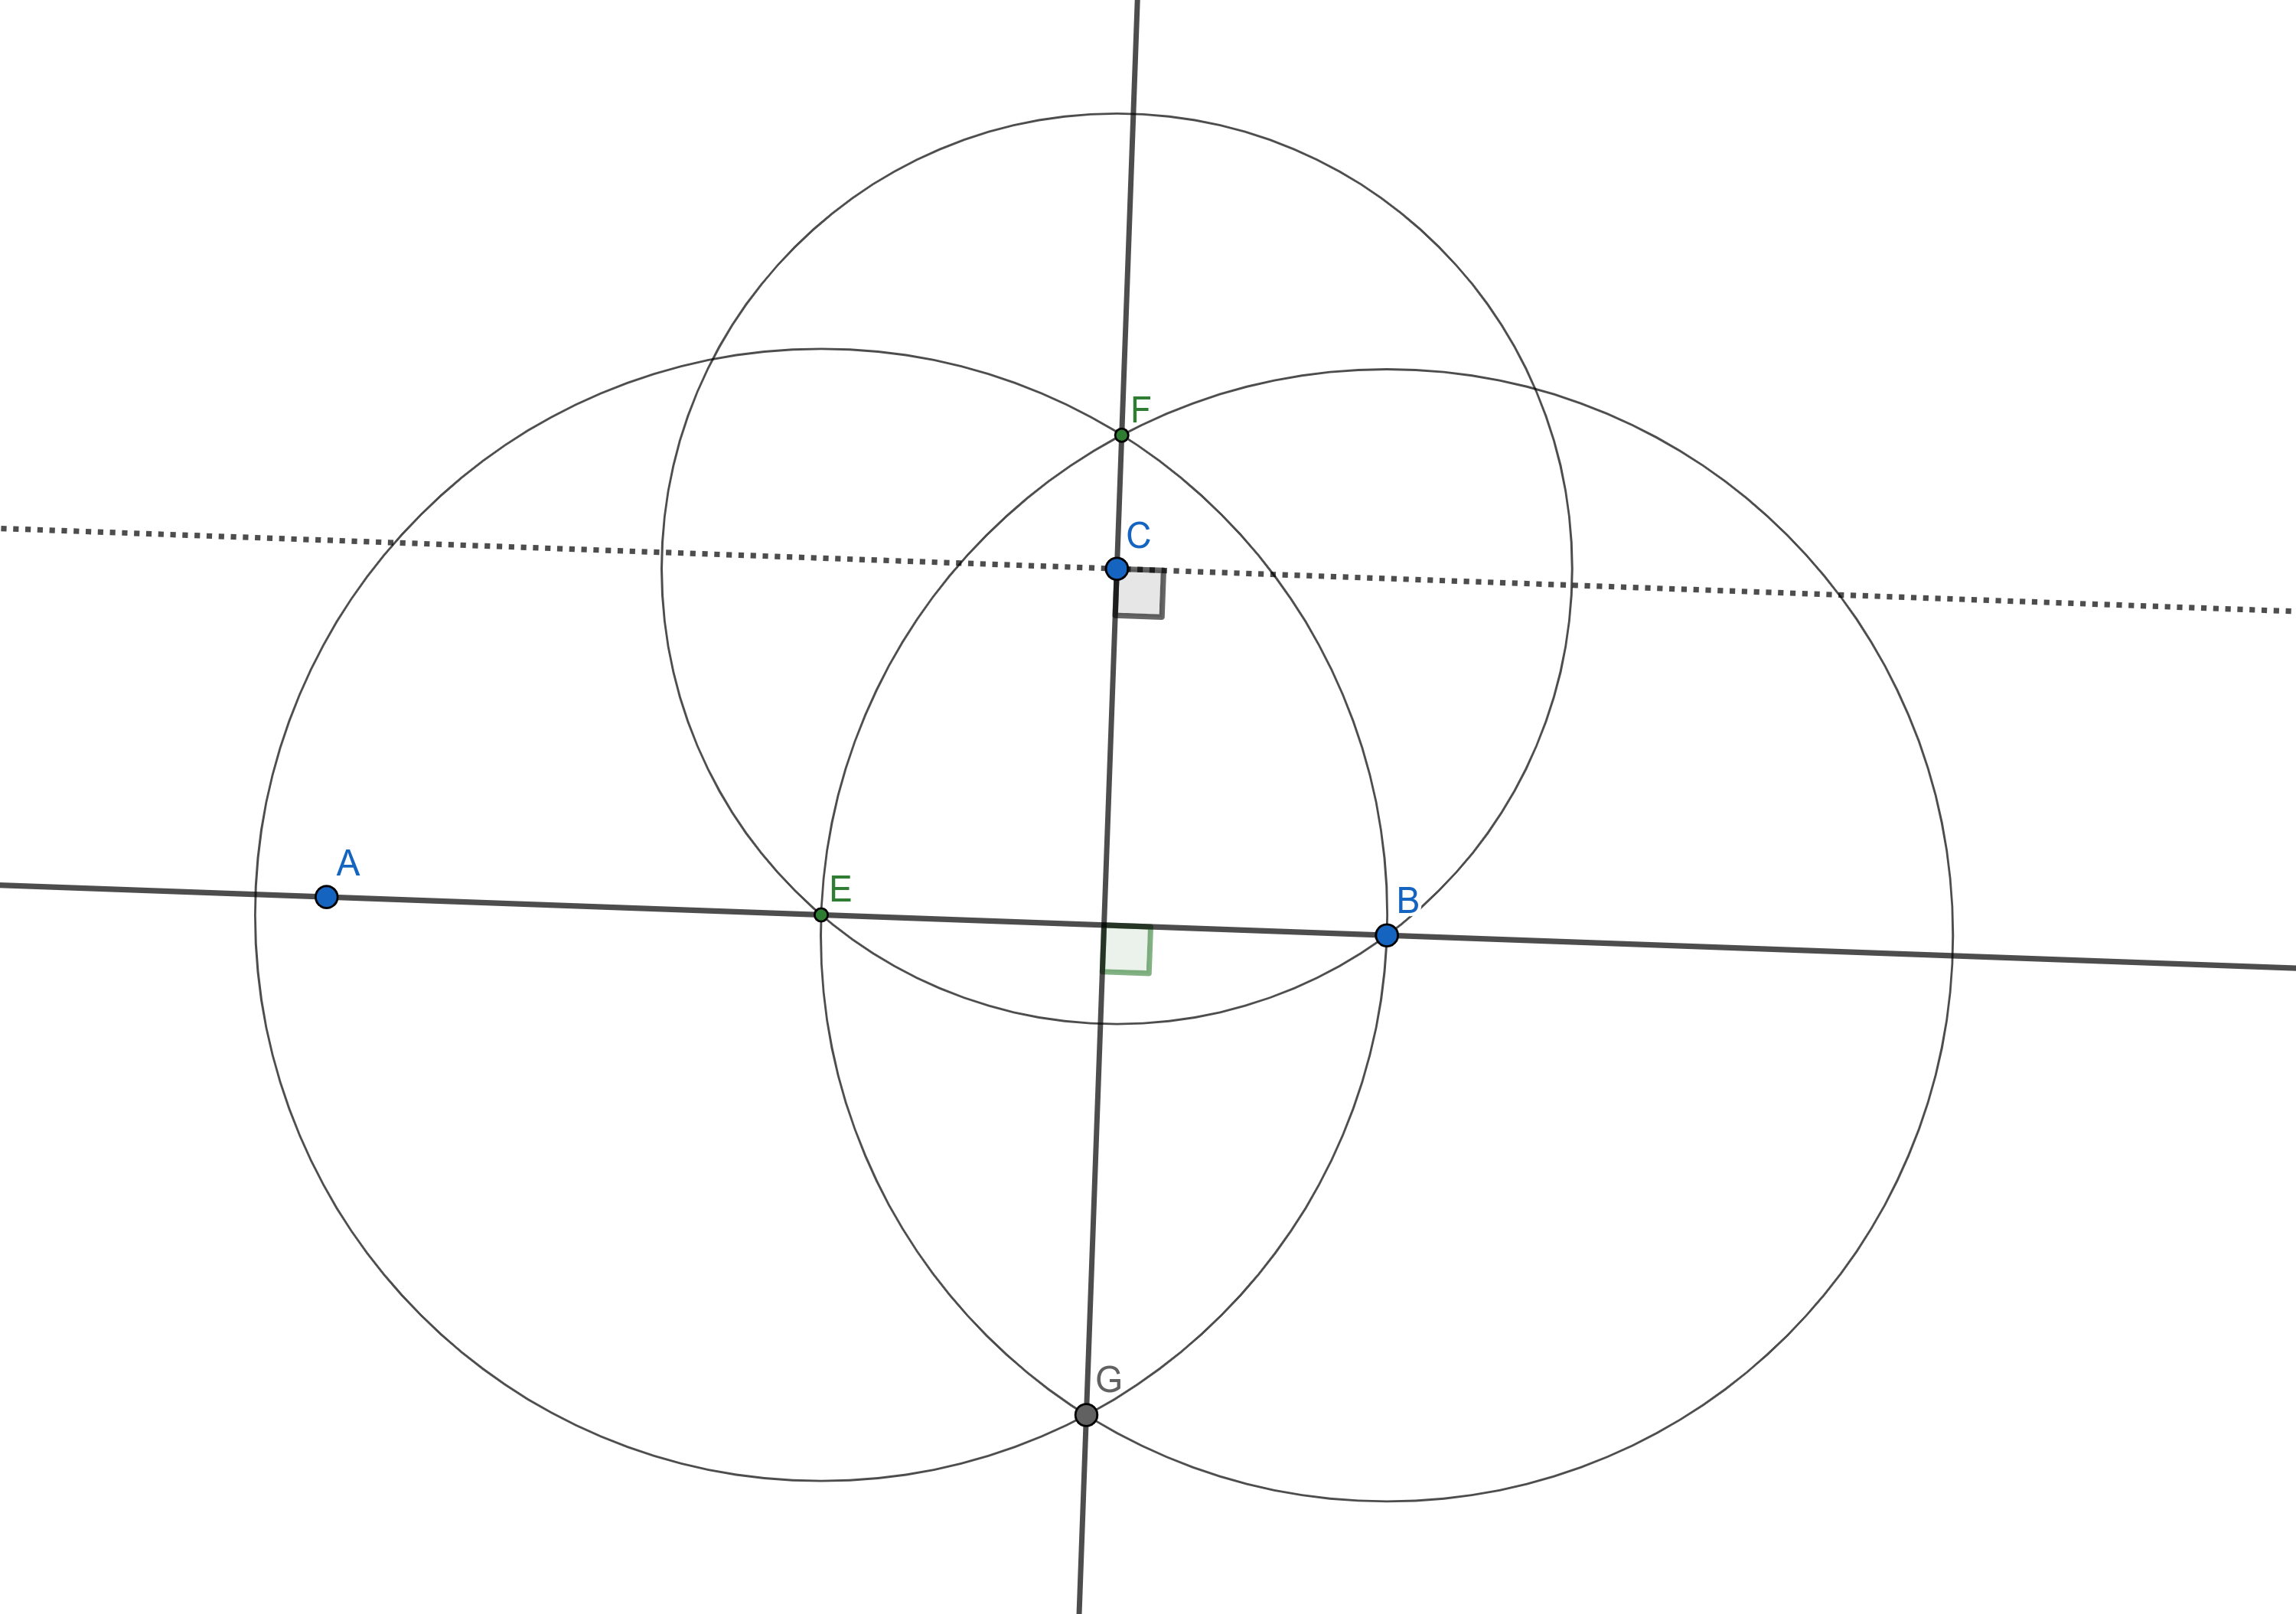
\includegraphics[width=0.9\textwidth]{perpendicular_parallel_.png}
        \end{center}
        \caption{A perpendicular can be dropped onto a line from any point, and a
        parallel line can be drawn through the point.}
        \label{fig:perpendicular_parallel}
        \end{figure}
    \end{frame}

    \begin{frame}
        \begin{figure}
        \begin{center}
            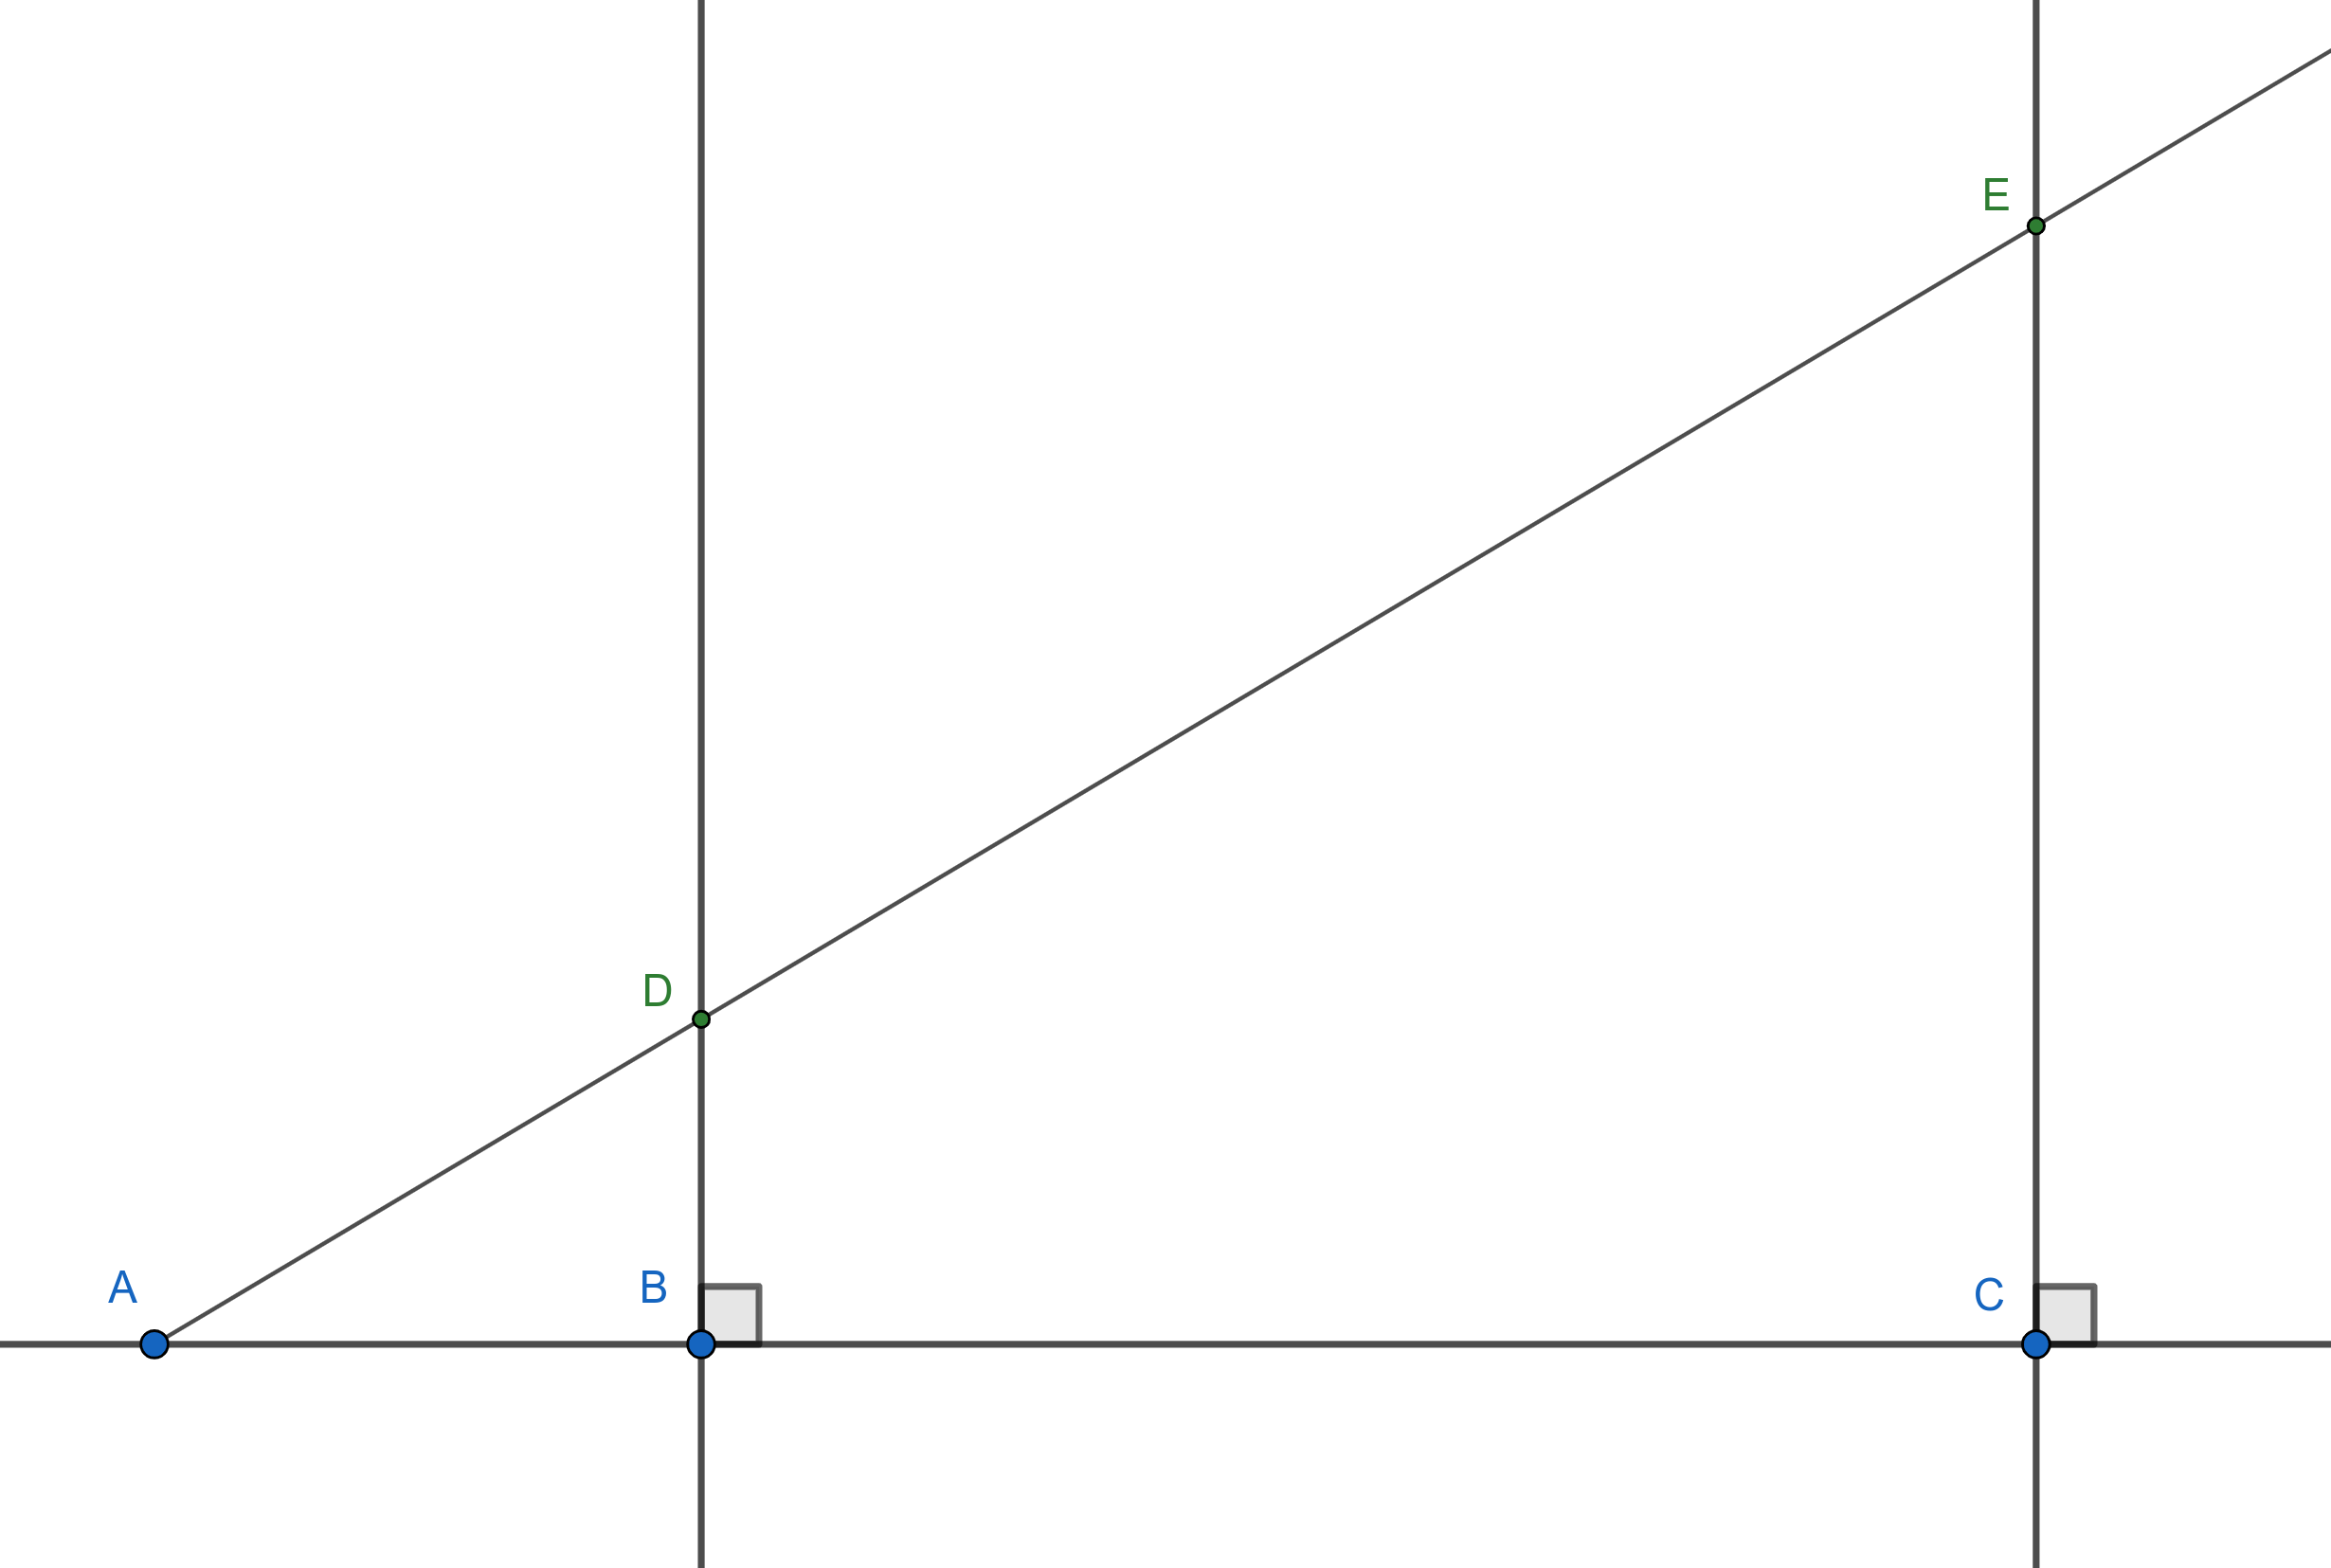
\includegraphics[width=0.9\textwidth]{multiply_divide_.png}
        \end{center}
        \caption{Any two lengths can be multiplied together or divided, via $DB =
        EC / AC$ with $AB = 1$.}
        \label{fig:multiply_divide}
        \end{figure}
    \end{frame}

    \begin{frame}
        \begin{figure}
        \begin{center}
            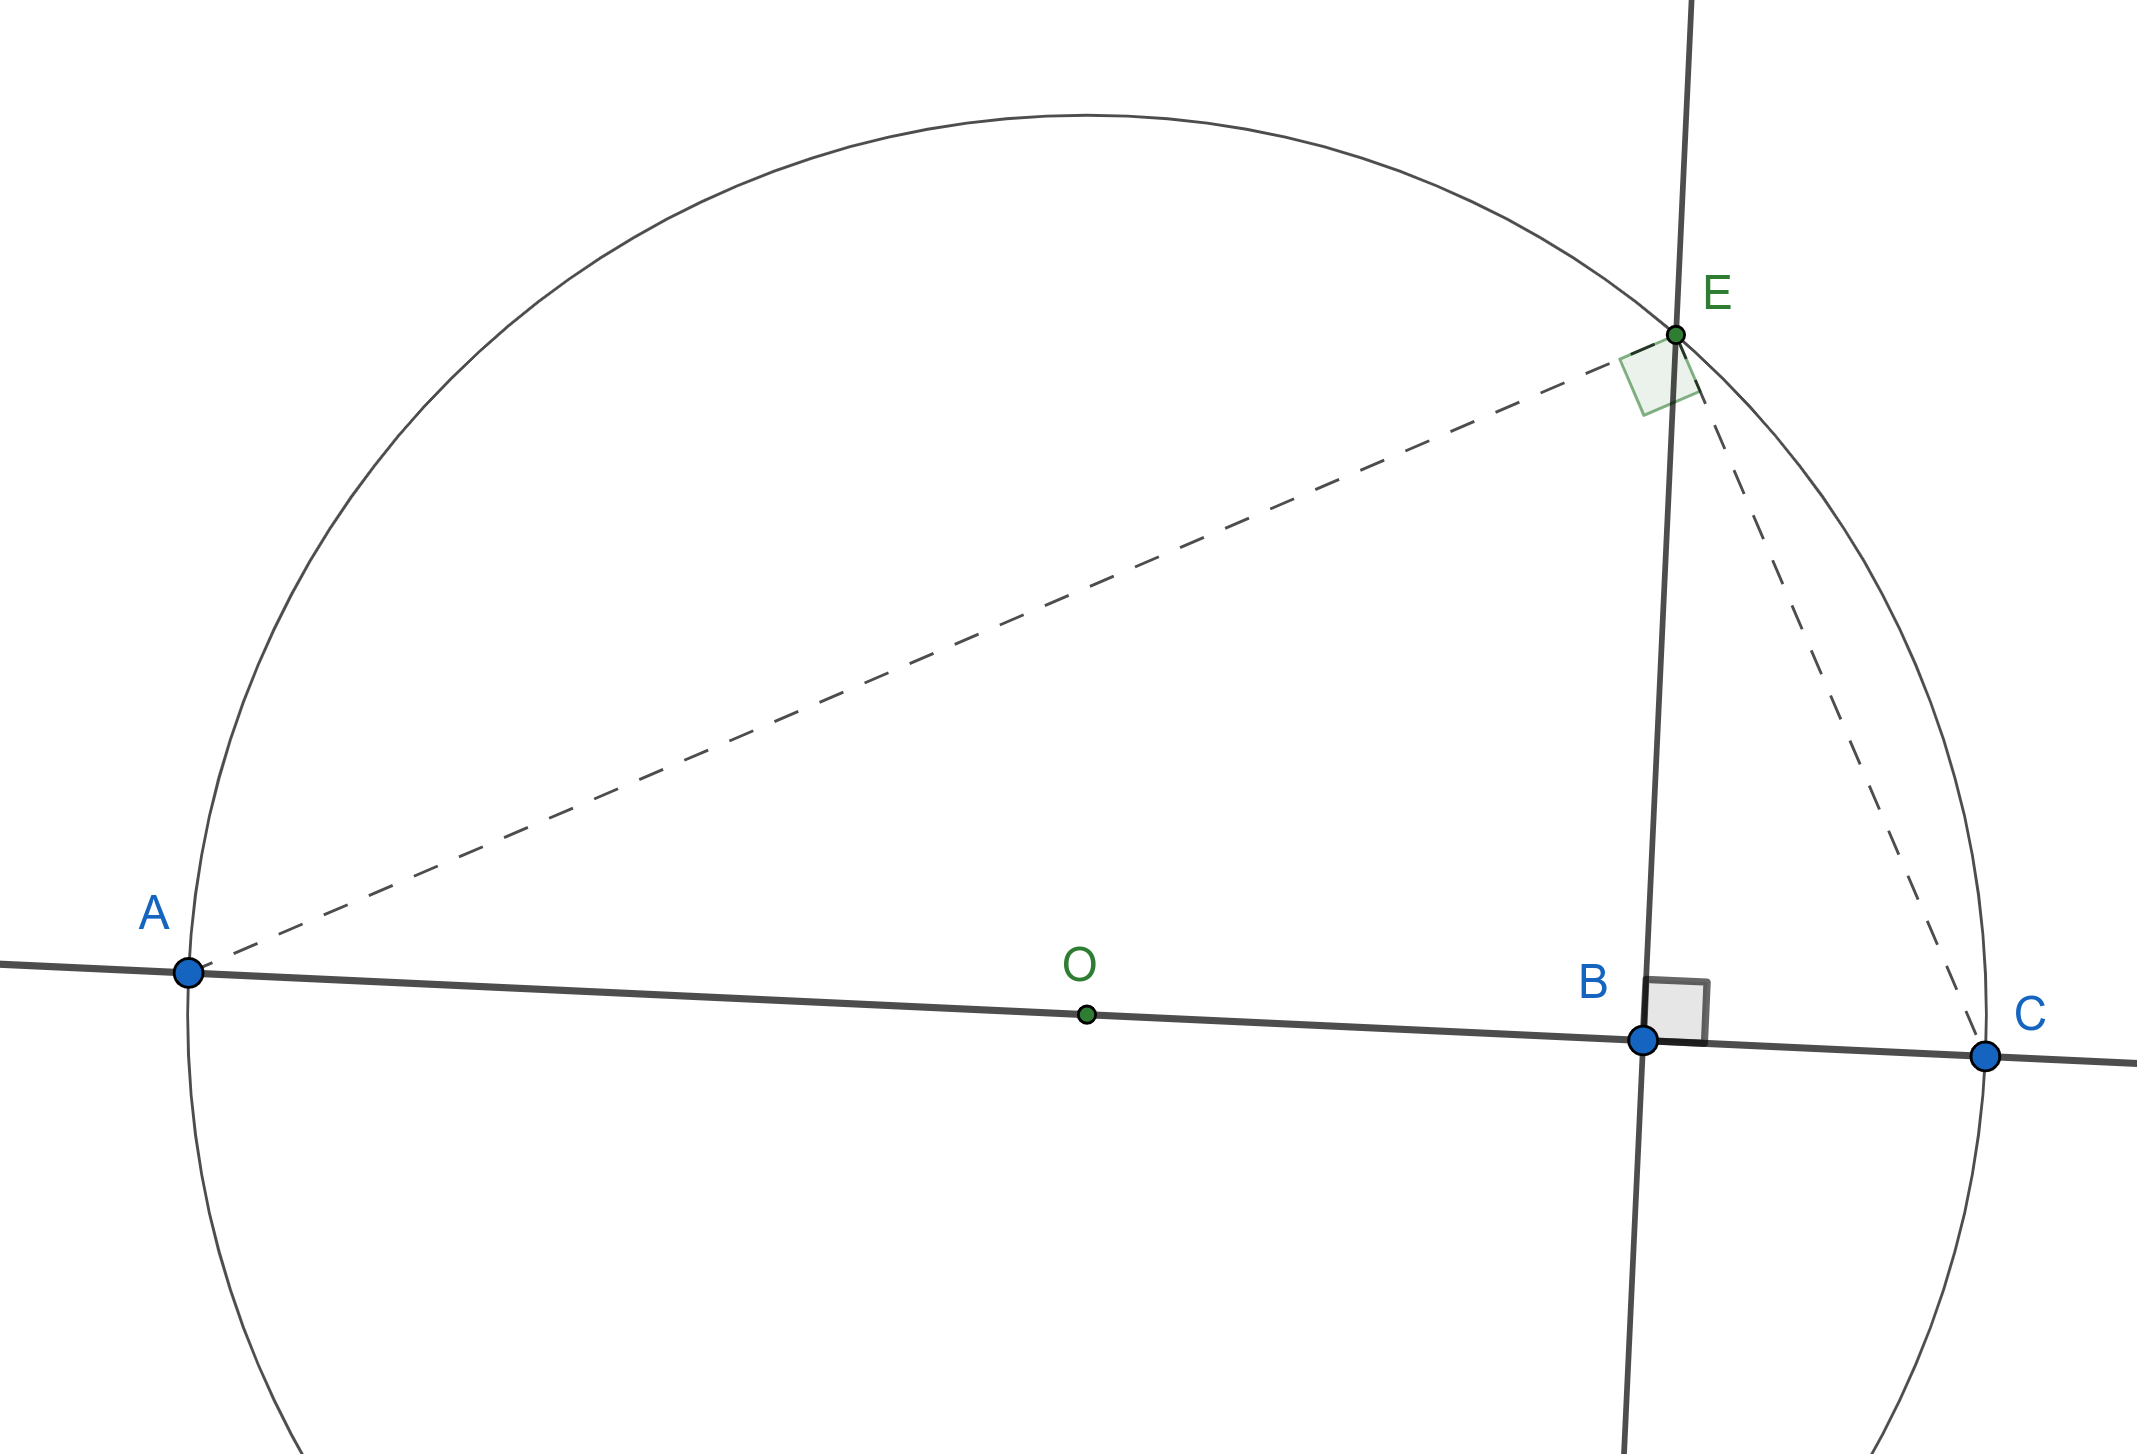
\includegraphics[width=0.9\textwidth]{square_root_.png}
        \end{center}
        \caption{The square root of any length can be constructed, via $AB = EB^2$
        with $BC = 1$.}
        \label{fig:square_root}
        \end{figure}
    \end{frame}

    \begin{frame}{Constructible numbers}
        Start by marking the points $0$ and $1$ on the complex plane. A number
        $\alpha \in \C$ is said to be constructible if and only if it can be
        constructed via straightedge and compass in finitely many steps.

        ~\\\pause
        \begin{block}{Remark} \vspace{0.1em}
            If $\alpha$ is constructible, so are
            $-\alpha$,
            $\overline{\alpha}$,
            $i\alpha$,
            $|\alpha|$,
            $\sqrt{\alpha}$,
            $\operatorname{Re}(\alpha)$,
            $\operatorname{Im}(\alpha)$.
        \end{block}
    \end{frame}

    \note[itemize]{
        \item Starting with $0$ and $1$, we can immediately construct the integers
        $\Z$, hence the field $\Q$.
    }

    \begin{frame}{Constructible numbers}
        Constructible numbers form a field.

        \begin{block}{Proof} \vspace{0.1em}
            If $\alpha$ and $\beta$ are constructible, so are $\alpha \pm \beta$,
            $\alpha\beta$, $\alpha / \beta$.
        \end{block}

        ~\\\pause
        \begin{block}{Remark} \vspace{0.1em}
            The field of constructible numbers contains $\Q$, and is contained within
            $\C$.
        \end{block}
    \end{frame}

    % \begin{frame}[standout]{}
    %     What can\only<2->{'t} we construct?
    % \end{frame}

    \section{The Language of Field Extensions}

    \begin{frame}{Field extensions}
        Let $F, K$ be fields with $F \subseteq K$. We say that $K/F$ is a field
        extension of $F$, also denoted $F \hookrightarrow K$.

        ~\\\pause

        With this, $K$ can be seen as an $F$-vector space. Define \[
            [K : F] = \operatorname{dim}_F(K).
        \]

        We say that $K/F$ is a \emph{finite extension} if $[K : F]$ is finite.
    \end{frame}

    \note[itemize]{
        \item The field of complex numbers $\C$ can be seen as a two dimensional
        vector space over $\R$.
    }

    \begin{frame}{Simple field extensions}
        Let $K/F$ be a field extension. Suppose that $\alpha \in K\setminus F$. Then,
        we define $F(\alpha)$ to be the smallest subfield of $K$ containing both $F$
        and $\alpha$.

        \[
            F(\alpha) = \left\{\frac{p(\alpha)}{q(\alpha)} : p, q \in F[x],\,
            q(\alpha) \neq 0\right\}.
        \]
    \end{frame}

    \begin{frame}{Algebraic extensions}
        We say that $\alpha$ is \emph{algebraic} over $F$ when $f(\alpha) = 0$ for
        some polynomial $f \in F[x]$.

        If $f$ is monic and of minimal degree, then $f$ is called the (unique)
        \emph{minimal polynomial} of $\alpha$.

        ~\\\pause

        \begin{exampleblock}{Examples} \vspace{0.1em}
            The minimal polynomial of $\sqrt{2}$ over $\Q$ is $x^2 - 2$.

            The minimal polynomial of $\sqrt[3]{2}$ over $\Q$ is $x^3 - 2$.

            The minimal polynomial of $\cos(\pi / 9)$ over $\Q$ is $x^3 - 3x/4 -
            1/8$.
        \end{exampleblock}
    \end{frame}

    \begin{frame}{Algebraic extensions}
        If $\alpha$ is algebraic over $F$, then \[
            F(\alpha) = \{p(\alpha) : p \in F[x]\} = F[\alpha].
        \] It follows that $[F(\alpha) : F]$ is precisely the degree of the minimal
        polynomial of $\alpha$ over $F$.

        \pause

        \begin{exampleblock}{Examples} \vspace{0.1em} \[ [\Q(\sqrt{2}) : \Q] = 2.
        \qquad [\Q(\cos(\pi / 9)) : \Q] =  3.  \] \end{exampleblock}

        \pause

        \begin{block}{Proof} \vspace{0.1em} The numbers $\{1, \alpha, \alpha^2,
        \dots, \alpha^{n - 1}\}$ form a basis of $F(\alpha)$.  \end{block}

        % \begin{block}{Proof} \vspace{0.1em} If $f$ is the minimal polynomial of
        % $\alpha$, then the evaluation map \[ F[x] \to F[\alpha], \qquad p \mapsto
        % p(\alpha) \] is a homomorphism of rings, with kernel $\langle f\rangle$.
        % Thus, $F[x]/\langle f \rangle \cong F[\alpha]$ is an isomorphism of fields.
        % Additionally, $F[\alpha] \subseteq F(\alpha)$.  \end{block}
    \end{frame}

    \note[itemize]{ \item Every element of $\Q(\sqrt{2})$ looks like $p(\sqrt{2})$;
    but every power of $\sqrt{2}$ is of the form $2^k$ or $2^k\sqrt{2}$. Thus, every
    element of $\Q(\sqrt{2})$ is of the form $a + b\sqrt{2}$.

        \item When $f$ is irreducible over $F$, then $\langle f\rangle$ is a maximal
        ideal in $F$.  }


    \begin{frame}{Chaining simple field extensions}
        Let $K/F$ be a field extension. Suppose that $\alpha_1, \dots, \alpha_k \in
        K\setminus F$. Then, we define $F(\alpha_1, \dots, \alpha_k)$ to be the
        smallest subfield of $K$ containing $F$ and all $\alpha_1, \dots, \alpha_k$.

        \begin{align*}
            F(\alpha_1, \dots, \alpha_k) &= F(\alpha_1, \dots,
            \alpha_\ell)(\alpha_{\ell + 1}, \dots, \alpha_k) \\
            &= F(\alpha_1)(\alpha_2)\dots(\alpha_k).
        \end{align*}
    \end{frame}

    \begin{frame}{Tower Lemma}
        Let $K/F$ and $L/K$ be finite field extensions. Then, $L/F$ is a finite field
        extension, with \[
            [L : F] = [L : K] [K : F].
        \]

        \pause

        \begin{exampleblock}{Example}
            \begin{align*}
                [\Q(\sqrt[3]{2}, \sqrt{3}) : \Q] &= [\Q(\sqrt[3]{2}, \sqrt{3}) :
                \Q(\sqrt{3})] [\Q(\sqrt{3}) : \Q] \\
                &= 3\times 2 = 6.
            \end{align*}
        \end{exampleblock}

        \pause

        \begin{block}{Proof} \vspace{0.1em}
            If $\{\alpha_1, \dots, \alpha_n\}$ is a basis of $K/F$ and $\{\beta_1,
            \dots, \beta_m\}$ is a basis of $L/K$, then $\{\alpha_1\beta_1, \dots,
            \alpha_i\beta_j, \dots, \alpha_n\beta_m\}$ is a basis of $L/F$.
        \end{block}
    \end{frame}

    % \begin{frame}{Tower Lemma}
    %     \begin{block}{Proof} \vspace{0.1em}
    %         If $\{\alpha_1, \dots, \alpha_n\}$ is a basis of $K/F$ and $\{\beta_1,
    %         \dots, \beta_m\}$ is a basis of $L/K$, then $\{\alpha_1\beta_1, \dots,
    %         \alpha_i\beta_j, \dots, \alpha_n\beta_m\}$ is a basis of $L/F$.

    %         Every $\gamma \in L$ can be expanded as \[
    %             \gamma = \sum_{j = 1}^m \gamma_j \beta_j = \sum_{j = 1}^m\sum_{i =
    %             1}^n \gamma_{ji} \alpha_i \beta_j,
    %         \] where $\gamma_j \in K$, $\gamma_{ji} \in F$. Furthermore, $\gamma = 0$
    %         forces each $\gamma_j = 0$, hence each $\gamma_{ji} = 0$.
    %     \end{block}
    % \end{frame}

    \begin{frame}{The field of constructible numbers}
        Constructible numbers form a field $\mathscr{C}$, with \[
            \Q(i) \subseteq \mathscr{C} \subseteq \C.
        \]

        ~\\\pause

        \begin{block}{Remark} \vspace{0.1em}
            If $\alpha$ is constructible, then so is $\sqrt{\alpha}$.
            Thus, $\mathscr{C}$ is a \emph{quadratically closed field} -- in
            particular, $\mathscr{C}$ is the \emph{quadratic closure} of $\Q$.
        \end{block}
    \end{frame}



    \section{The Constructible Number Theorem}

    \begin{frame}{Minimal polynomials of constructible numbers}
        If a number $\alpha \in \C$ is constructible, then $[\Q(\alpha) : \Q] = 2^n$
        for some integer $n$.

        Equivalently, the degree of the minimal polynomial of $\alpha$ over $\Q$ must
        be a power of $2$.

        ~\\\pause

        \begin{exampleblock}{Example} \vspace{0.1em}
            The number $\cos(\pi/9)$, hence the angle $\pi / 9$, is not
            constructible.

            The number $\sqrt[3]{2}$ is not constructible.

            The number $\sqrt{\pi}$ is not even algebraic!
        \end{exampleblock}
    \end{frame}


    \begin{frame}{Lines and circles}
        If $\alpha$ lies at the intersection of some lines $L(\beta_i, \delta_i)$
        and/or circles $C(\gamma_i, R_i)$ for some $\beta_i, \delta_i, \gamma_i, R_i
        \in F$ where the field $F\supseteq \Q$ is closed under conjugation, then
        \[
            [F(\alpha) : F] \leq 2.
        \]

        \pause

        In other words, there exist $\xi, \zeta \in F$ such that \[
            \alpha^2 - 2\xi\alpha + \zeta = 0 \;\Longleftrightarrow\;
            \alpha = \xi \pm \sqrt{\xi^2 - \zeta}.
        \]

        % \begin{block}{Remark} \vspace{0.1em}
        %     $\beta = s + it \in F$ gives $s, t, |\beta|^2 \in F$.
        % \end{block}
    \end{frame}

    \note[itemize]{
        \item In the beginning, we only have the numbers $0$ and $1$, which are
        contained in the field $\Q$.

        \item After finitely many steps, i.e.\ after drawing finitely many
        lines/circles, we have finitely many new points (located at intersections of
        lines/circles). These are all contained in some field $F$, with $\Q \subseteq
        F \subseteq \C$.

        \item Now, any new line/circle has parameters from $F$. Thus, any new point
        constructed at this step is at the intersection of lines/circles with
        parameters from $F$.
    }


    \begin{frame}{Intersection of two lines}
        The lines $\beta_i + (\delta_i - \beta_i)x \equiv \beta_i + \gamma_i x$
        intersect at \[
            \beta_1 + \gamma_1 \frac{v_2(s_2 - s_1) + u_2(t_1 - t_2)}{u_1v_2 -
            u_2v_1},
        \] where $\beta_i = s_i + it_i$, $\gamma_i = u_i + iv_i$.

        % \pause

        \begin{block}{Proof} \vspace{0.1em}
            Solve the system \[
                s_1 + u_1x_1 = s_2 + u_2x_2, \qquad t_1 + v_1x_1 = t_2 + v_2x_2.
            \]
        \end{block}
    \end{frame}


    \begin{frame}{Intersection of a line and a circle}
        The line $\beta + \delta x$ and the circle $|z - \gamma|^2 = R^2$
        intersect at \[
            \beta + \delta x
        \] where $x$ is a real root of the quadratic \[
            |\delta|^2 x^2 + \left[(\beta - \gamma)\overline{\delta} +
            \overline{(\beta - \gamma)}\delta\right]x = R^2 - |\beta - \gamma|^2.
        \]

        % \pause

        \begin{block}{Proof} \vspace{0.1em}
            Expand \[
                |(\beta - \gamma) + \delta x|^2 = R^2.
            \]
        \end{block}
    \end{frame}

    \begin{frame}{Intersection of two circles}
        The circles $|z - \gamma_i|^2 = R_i^2$ intersect at \[
            x + iy
        \] where \[
            2(u_1 - u_2)x + 2(v_1 - v_2)y = R_2^2 - R_1^2 + |\gamma_1|^2 -
            |\gamma_2|^2,
        \] and $\gamma_i = u_i + iv_i$.

        % \pause

        This reduces to the previous case!
    \end{frame}

    \begin{frame}{Building a tower}
        Let $\alpha$ be constructible. There is a finite sequence of lines and
        circles such that the final diagram has $\alpha$ at some intersection.

        \pause

        Look at the diagram at step $m$. There are finitely many intersections of
        lines and circles present, say $\alpha_1, \dots, \alpha_k$. Thus, they all
        lie in the field $\Q(\alpha_1, \dots, \alpha_k) = F_n$.

        \pause

        In the next step, a line or circle is drawn using these existing points, so
        any new intersection $\alpha_{k + i}$ must lie in $F_m(\alpha_{k + i})$ with
        $[F_m(\alpha_{k + i}) : F_m] \leq 2$.
    \end{frame}

    \begin{frame}{The constructible number theorem}
        A number $\alpha \in \C$ is constructible \emph{if and only if} $\alpha$ lies
        in an \emph{iterated quadratic extension} of $\Q$, i.e.\ there exists a tower
        of fields \[
            \Q = F_0 \hookrightarrow F_1 \hookrightarrow \dots \hookrightarrow F_{n -
            1} \hookrightarrow F_n
        \] with each $[F_j : F_{j - 1}] = 2$ and $\alpha \in F_n$.
    \end{frame}

    \begin{frame}{The constructible number theorem}
        \begin{block}{Proof of converse} \vspace{0.1em}
            Suppose that every number from $F_{j - 1}$ is constructible.
            If $[F_j : F_{j - 1}] = 2$, then $F_j/F_{j - 1}$ has a basis of the form
            $\{1, \beta\}$, where \[
                \beta^2 - 2\xi\beta + \zeta = 0 \;\Longleftrightarrow\;
                \beta = \xi \pm \sqrt{\xi^2 - \zeta}
            \] for some $\xi, \zeta \in F_{j - 1}$. This means that $\beta$ is
            constructible, since $\mathscr{C}$ is quadratically closed.

            Consequently, every $\alpha \in F_j$ is constructible, since it can be
            written in the form $\alpha = \gamma + \delta\beta$ for $\gamma, \delta
            \in F_{j - 1}$.
        \end{block}
    \end{frame}


    \section{Bending the Rules}

    \begin{frame}
        \begin{figure}
            \centering
            \begin{subfigure}
                \centering
                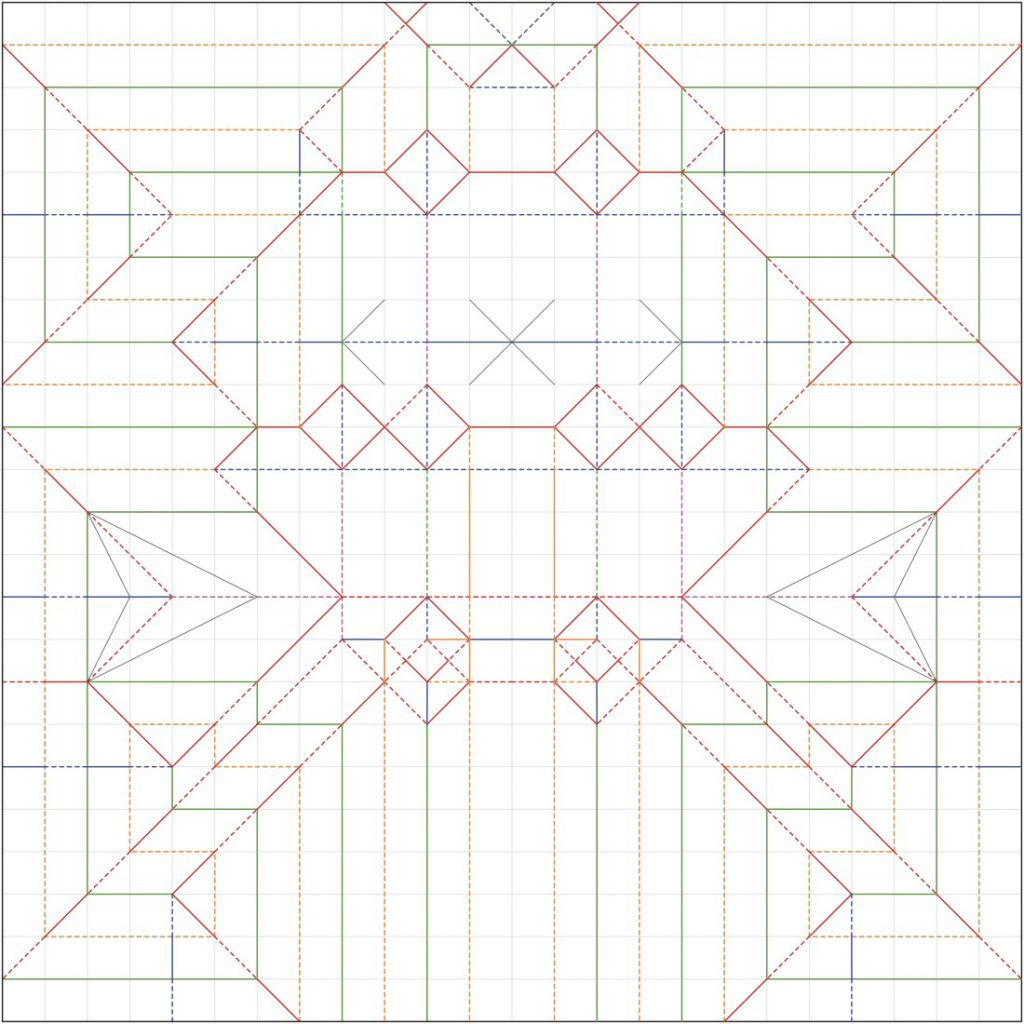
\includegraphics[width=0.54\linewidth]{scarab_pattern.jpg}
            \end{subfigure}
            \begin{subfigure}
                \centering
                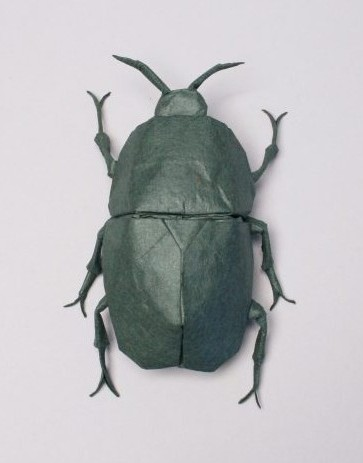
\includegraphics[width=0.43\linewidth]{scarab.jpg}
            \end{subfigure}
            \caption{Scarab with Elytra, \emph{Opus 594}, Robert J. Lang.}
            \label{fig:scarab}
        \end{figure}
    \end{frame}

    \begin{frame}{Origami constructions: Huzita-Hatori}
        \begin{enumerate}
            \item A line can be drawn through any two constructed points.
            \item The perpendicular bisector of any two constructed points can be
            drawn.
            \item The angle bisector of any constructed angle can be drawn.
            \item The perpendicular to any constructed line through any constructed
            point can be drawn.
            \item Given a constructed line $L$ and constructed points $\alpha,
            \beta$, a line through $\beta$ that reflects $\alpha$ onto $L$ can be
            drawn.
            \item \alert<2->{Given constructed lines $L, M$ and constructed points
            $\alpha, \beta$, a line that simultaneously reflects $\alpha$ onto $L$
            and $\beta$ onto $M$ can be drawn.}
        \end{enumerate}
    \end{frame}

    \note[itemize]{
        \item Hatori showed that the first five axioms can be recovered from the
        sixth.

        \item Robert Lang showed that these are complete.

        \item The first five axioms give a system equivalent to compass and
        straightedge constructions.

        \item The sixth axiom has a similar effect as that of a marked ruler.

        \item With this, one can find a simultaneous tangent to two parabolas, hence
        solve cubic equations.
    }

    \begin{frame}{The origami constructible number theorem}
        A number $\alpha \in \C$ is origami constructible \emph{if and only if} there
        exists a tower of fields \[
            \Q = F_0 \hookrightarrow F_1 \hookrightarrow \dots \hookrightarrow F_{n -
            1} \hookrightarrow F_n
        \] with each $[F_j : F_{j - 1}] = 2$ or $3$, and $\alpha \in F_n$.

        ~\\\pause

        \begin{block}{Remark} \vspace{0.1em}
            This means that $[\Q(\alpha) : \Q] = 2^n3^m$ for some integers $n, m$.
        \end{block}
    \end{frame}

    \begin{frame}
        \vspace{0.5em}
        \begin{figure}
        \begin{center}
            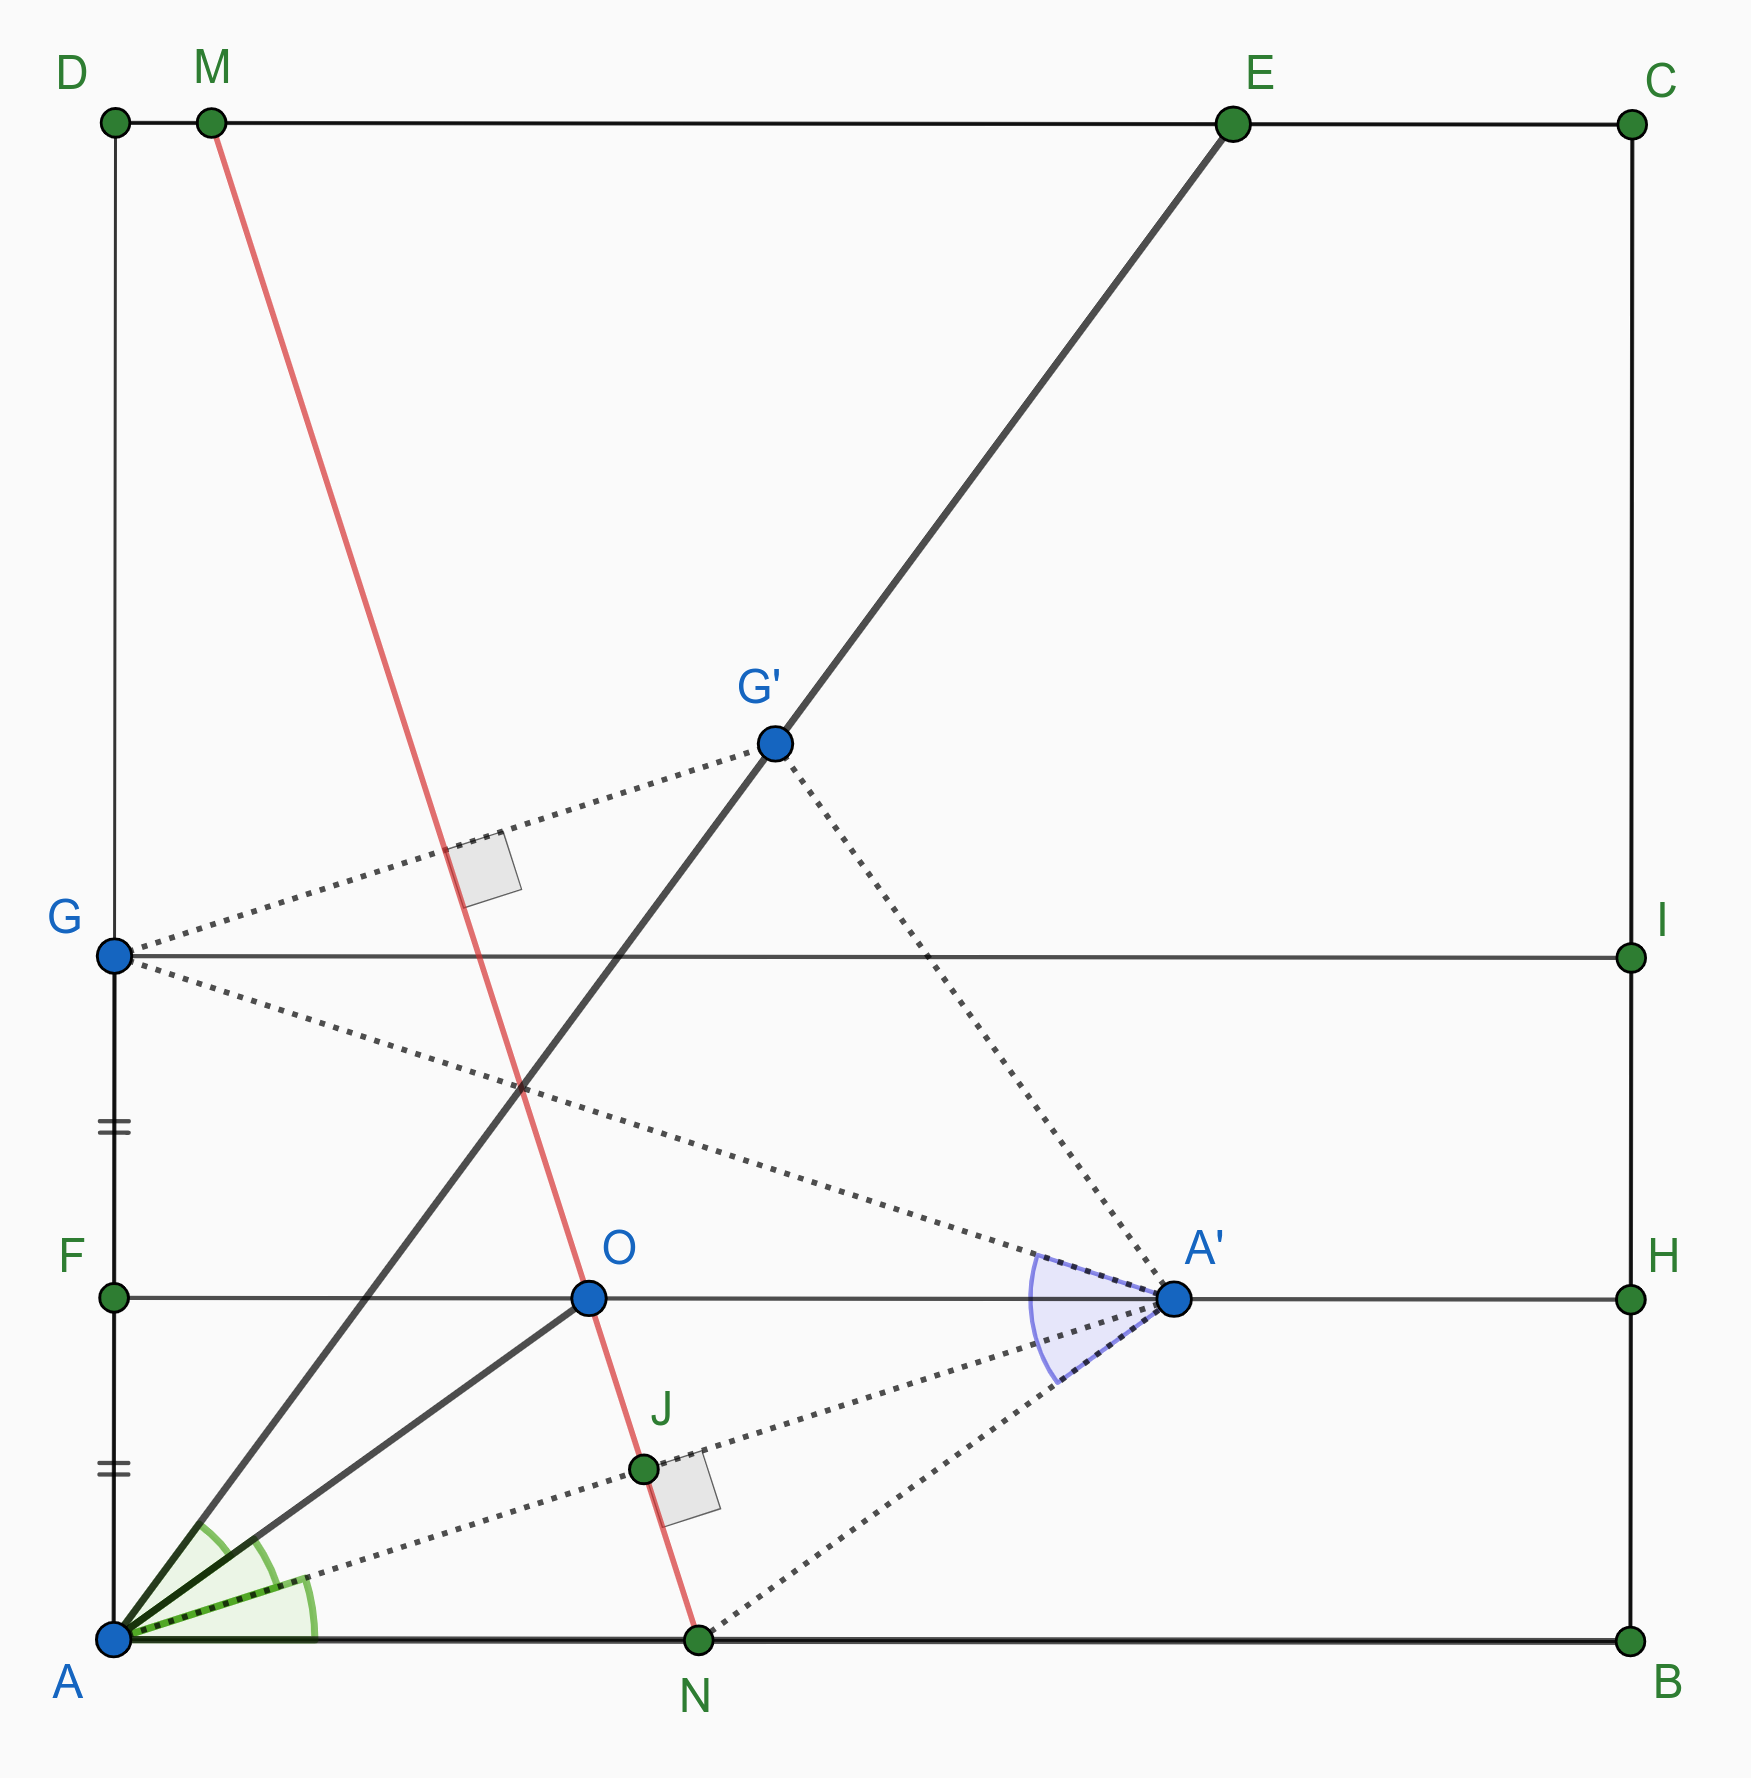
\includegraphics[width=0.7\textwidth]{trisection_origami_.png}
        \end{center}
        \vspace{-0.5em}
        \caption{Using Origami to trisect the angle $\angle EAB$}
        \label{fig:trisecting_angles_origami}
        \end{figure}
    \end{frame}


    \begin{frame}{References}
        \nocite{*}
        \bibliography{references}
        \bibliographystyle{plain}
    \end{frame}

\end{document}
